\documentclass[12pt]{article}
\usepackage{amsmath, amssymb, graphicx}
\usepackage[a4paper, margin=1in]{geometry}
\usepackage{booktabs} 
\usepackage{multirow}

\begin{document}

\begin{titlepage}
    \centering
    \vspace*{1in}
    
    {\LARGE \textbf{The electromagnetic graviton}}\\[1.5cm]
    
    {\large Alexandre Furtado Neto}\\[0.5cm]
    {Corresponding Author: alexandre.com@yahoo.com}\\
    {Mailing Address: Rua Escritor Rodrigo Melo Franco, 400, ap. 2/1003, 22783-124, Rio de Janeiro, Brazil}\\[1.5cm]
    
    {\large March 31, 2025}\\[1.5cm]
    
    \textbf{Abstract}\\[0.5cm]
    \begin{minipage}{0.9\textwidth}
        \small
This essay explores the gravitational aspects of a toy universe constructed as a discrete cellular automaton. The model consists of a layered 3D toroidal lattice where fundamental interactions emerge from structured bit-encoded properties. Gravity is proposed to arise from a class of paired wavefronts termed \textit{gravitons}, which mediate residual attractive forces through their interaction across distinct sectors of the system. Unlike conventional force carriers, gravitons exhibit dual-sector coupling, enabling energy redistribution and a phenomenon analogous to dark matter. The model's discrete dynamics preserve relativistic properties, providing a framework for emergent spacetime structures. Through the interplay of charge coherence, sinusoidal modulation, and spatial diffusion, this study suggests an alternative perspective on gravity as a residual effect of electromagnetic-like interactions.
    \end{minipage}\\[1.5cm]
    
    \textit{Essay written for the Gravity Research Foundation 2025 Awards for Essays on Gravitation.}
\end{titlepage}   

\section{Introduction}
This essay explores the gravitational aspects of a toy universe currently being developed in \cite{ResearchGate}. First, we summarize the key features of the model. Then, in Section \ref{emergence}, we highlight its novelty by identifying its gravitational origins.

The central idea is that physical reality can be understood in terms of discrete binary choices, aligning with Wheeler's "it from bit" concept. Information is considered fundamental to physics, though its ontological nature remains elusive. This work adopts a cellular automaton (CA) framework. Cellular automata, with their discrete evolution rules, provide a computationally accessible way to model physical systems. Unlike previous abstract or limited models, this research proposes a full 3+1 dimensional core specification, allowing for direct computational analysis. The objective is not to claim that the universe operates as a CA but to use it as a useful representation for exploring fundamental physical laws.

The motivation behind this approach is the long-standing challenge of unifying Quantum Mechanics and General Relativity into a theory of quantum gravity. The study suggests that the presence of imaginary numbers in Schrödinger’s equation and the spacetime metric creates an epistemological barrier to this unification. By constructing a framework based solely on classical logic, bits, and topology, the research offers an alternative perspective on fundamental physics. The historical coincidence of Schrödinger’s equation and the Born rule revolutionized quantum mechanics, yet the debate over the true nature of reality continues. This work seeks to move beyond mere interpretation by proposing a deeper, constructive description of nature, acknowledging operator mechanics as a necessary tool in this endeavor.

\section{Space and Time}
Space consists of a 3D toroidal lattice of size $L$, with an extra non-spatial dimension of size $W$ forming a layered structure. Each cell stores a structured bit string encoding physical properties such as charge, motion, and affinity. Time is discrete and unidirectional, progressing in uniform steps.

The affinity property is essential for the formation of composite structures; without it, only a holistic universe would emerge. It is also the substrate for the emergent phenomenon of entanglement and characterizes the track left by the particles in self-interference.

\subsection{Cell Structure}
The cell structure is shown in Table \ref{tab:Cell-structure}.

\subsection{The Lattices}
Three interlaced lattices (main, draft, and mirror) ensure proper data handling and interactions.

\begin{table}
\begin{centering}
\begin{tabular}{|l|c|l|l|}
\hline 
\textbf{\large{}Name} & \textbf{\large{}Type} & \textbf{\large{}Symbol} & \textbf{\large{}Obs.}\tabularnewline
\hline 
\hline 
\multicolumn{4}{|c|}{\textbf{Physical properties}}\tabularnewline
\hline 
charge & B6 & \emph{ch} & bits $q$, $w_{1}$, $w_{0}$, $c_{2}$, $c_{1}$, $c_{0}$\tabularnewline
\hline 
route & B & $p$ & linear motion direction bit\tabularnewline
\hline 
twist & B & $\bar{p}$ & rotation spiral bit\tabularnewline
\hline 
affinity & N & $a$ & groups bubbles into particles\tabularnewline
\hline 
position & V & $\boldsymbol{x}$ & spatial coordinates\tabularnewline
\hline 
\multicolumn{4}{|c|}{\textbf{Wavefront}}\tabularnewline
\hline 
Euclidean distance & DN & \emph{d} & for spherical constraint\tabularnewline
\hline 
sine mask & B & \emph{s} & fixed period mask bit\tabularnewline
\hline 
wavefront tick & DN & $t$ & light clocking\tabularnewline
\hline 
sine timing & DN & $\theta$ & independent time for sine (arc)\tabularnewline
\hline 
\multicolumn{4}{|c|}{\textbf{Operational variables}}\tabularnewline
\hline 
relocation offset & V & \textbf{\emph{c}} & determines reissue address\tabularnewline
\hline 
housekeeping tick & DN & $k$ & timeless clocking\tabularnewline
\hline 
collapse flag & B & $col$ & hints collapse\tabularnewline
\hline 
\end{tabular}
\par\end{centering}
\caption{Cell structure.}
{\small{}The formatted bit string is valid for all cells, where }\emph{\small{}N}{\small{}
represents a natural number, }\emph{\small{}DN}{\small{} 
a double natural number, }\emph{\small{}V}{\small{} a three-dimensional natural vector, and }\emph{\small{}B}{\small{} 
a boolean. The conventions for the values }\emph{\small{}false}{\small{} and }\emph{\small{}true}{\small{} for each 
charge bit are as follows: $q$: }\textbf{\small{}+}{\small{}, }\textbf{\small{}-}{\small{}; $w_{1}$: {[}$O${]}rbis, {[}$D${]}ark; 
$w_{0}$: {[}$R${]}ight, {[}$L${]}eft; $c_{2}$: {[}$B${]}lue, anti{[}$\bar{B}${]}lue; $c_{1}$: {[}$G${]}reen, anti{[}$\bar{G}${]}reen; 
$c_{0}$: {[}$R${]}ed, anti{[}$\bar{R}${]}ed.}\label{tab:Cell-structure}
\end{table}

\section{Fundamental Patterns}
A bubble is an expanding wavefront propagating spherically, dictated by Euclidean distance and a sinusoidal mask. Bubbles undergo relocation upon interaction, ensuring causality and preserving the speed of light. Charge types influence motion and interactions, while route and twist bits define linear and rotational dynamics.

Two superposing bubbles can form a \emph{pair} if they share a common affinity value. When two bubbles form a pair, the action of their weak or strong charges (but not the electric charge) is inhibited if they are complementary. Both bubbles are reissued in an interaction involving a pair. In general, the combinations formed correspond to boson fragments. A bubble that does not form a pair is called a \textit{singleton}.

By the simple fact that $W$ is an odd number, if we try to form pairs from different layers, an ultimate singleton will automatically remain. Let's call it the \textit{rebel}. The rebel will play an important role in breaking the original symmetry of this toy universe.

Finally, pairs that exhibit all complementary charge characteristics are termed \emph{gravitons}. These pairs can operate in both Orbis and Umbra.\footnote{Clearly, Orbis and Umbra coexist spatially.}. Each graviton pair has a fixed, absolute, oscillation frequency of 2, corresponding to their fundamental resonance in this dual framework. Gravitons contribute to the static interactions in both sectors. Without the graviton, matter from Umbra would appear entirely inert, and gravity would not exist. 

\subsection{Sine Sieve}
A squared sine function modulates interactions, resembling quantum probability distributions.

\subsection{Spiral Pattern}
The model encodes rotational dynamics through a canonical spiral pattern (Figure~\ref{fig:spiral}), initialized using a modified Archimedean spiral with parametric equations:
\begin{align}
    r &= \frac{L}{4\pi}\theta, \nonumber \\
    x &= r\cos(\theta) + \frac{L}{2}, \nonumber \\
    y &= r\sin(\theta) + \frac{L}{2}, \nonumber \\
    z &= r + \frac{L}{2}. \label{eq:spiral}
\end{align}
Here, \( \theta \) spans \( 2\pi \) radians, and \( L \) is the lattice size. The spiral’s points are mapped to cells via rotation matrices derived from orthogonal bases (Sec.~5.7), activating the twist bit \( \bar{p} \) in selected cells. 

This spiral serves two critical roles:
\begin{itemize}
    \item \textbf{Rotation \& Polarization}: The twist bit \( \bar{p }\) drives spatial rotations and photon polarization, mimicking spin-1 behavior in quantum systems.
    \item \textbf{Relativistic Consistency}: The orthogonal alignment of spirals to route lines (\( p \)) ensures Lorentz-like symmetry, preserving causal structure despite discrete mechanics.
\end{itemize}

\begin{figure}[htbp]
    \centering
    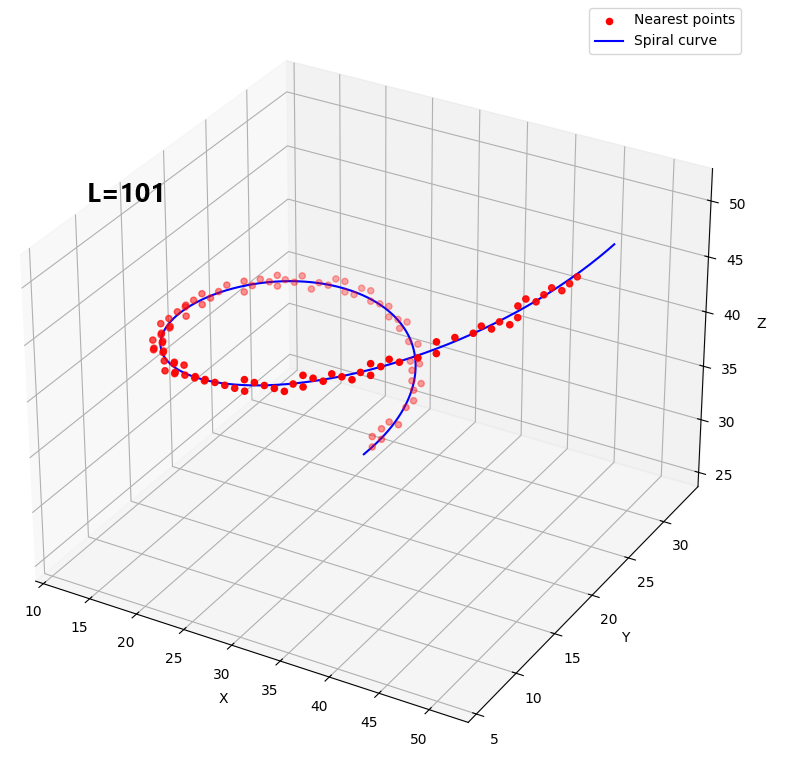
\includegraphics[width=0.6\textwidth]{fig3}
    \caption{The canonical spiral (Eq.~\ref{eq:spiral}) governing rotational dynamics. Points marked in red activate the twist bit \( \bar{p} \), inducing emergent angular momentum.}
    \label{fig:spiral}
\end{figure}


\subsection{Relativity Considerations}
The model's discrete mechanics approximate Minkowski spacetime properties, preserving interval invariance and causality.

\section{Particles}
Particles form from bubble aggregates sharing affinity values. The system supports fermions, bosons, and specialized pairs:
\begin{itemize}
    \item \textbf{Fermions}: Particles with unpaired kinematic components, confined by charge cohesion.
    \item \textbf{Bosons}: Fully paired bubbles, forming photons and gauge bosons.
    \item \textbf{Gravitons}: Special pairs mediating a static attractive force resembling gravity.
\end{itemize}

\section{Initial State}
The universe originates from a singularity where all bubbles overlap. Initialization follows structured rules, ensuring isotropic charge and motion distribution. Quantization effects arise from lattice constraints, influencing charge conservation and particle stability.

\section{The Light Frame}
The model operates as a cellular automaton finite state machine (FSM), progressing through four phases:
\begin{enumerate}
    \item \textbf{Convolution}: Bubbles interact based on charge compatibility and wavefront conditions.
    \item \textbf{Diffusion}: Interaction results propagate across layers.
    \item \textbf{Relocation}: Bubbles shift to maintain causality.
    \item \textbf{Transport}: Motion updates maintain time evolution.
\end{enumerate}
Charge conjugation ensures conservation laws, and interactions are governed by simple logical rules.

\section{Interaction Details}
Key interactions include:
\begin{itemize}
    \item \textbf{Charge Dynamics}: Charge-conserving rules dictate particle transformations.
    \item \textbf{Coulomb and Magnetic Forces}: Static fields arise from bubble alignments with gravitons.
    \item \textbf{Self-Interference}: Memory effects in space enable quantum-like interference.
\end{itemize}

\section{Discussion} \label{emergence}
The model posits that gravity arises as a residual effect of electromagnetic interactions, emerging naturally within the cellular automaton framework through the interplay of photons and gravitons. Acting as super photons, gravitons possess properties that allow them to mediate interactions across the two overlapping sectors of the toy universe, \emph{Orbis} and \emph{Umbra}. While ordinary photons are restricted to sector-specific interactions, gravitons provide a mechanism for fundamental connectivity in a universe otherwise marked by a strong separation between these domains. However, their direct influence on distant masses diminishes due to the cancellation of antagonistic forces induced by their interactions. What remains is a residual, geometry-driven attractive force that underpins the emergent gravitational effect. Through this dual-sector capability, gravitons redistribute energy and charge, also contributing to phenomena analogous to dark matter.

The model also suggests that the quantization of gravity must be sought, not at the microscopic level, as usual, but at a cosmological scale. Quantization of the electric charge comes from the cited topological monopole. The strong quantization comes from the combined action of electric and color exchange rules, manifested by the existence of hadrons. The quantization induced by the (relatively rare) weak interactions manifests itself at a cosmological scale: the relation between the average distance between galaxies and their bulges is constant. The large-scale granularity could then also be interpreted as a gravitational quantization.

\section{Conclusion}
This toy universe model offers a discrete, information-theoretic framework for emergent gravity, where gravitons mediate residual attractive forces through dual-sector interactions. By grounding physics in cellular automaton dynamics, the approach sidesteps the need for imaginary numbers or continuous spacetime, addressing key epistemological barriers in quantum gravity. The model’s falsifiability hinges on experimental tests of self-interference mechanisms—e.g., if electrons were shown to physically traverse both paths in a double-slit experiment, the trace-based interference proposed here would be invalidated. While undecidability challenges long-term predictions, the framework provides a concrete pathway to explore unification without abandoning determinism or locality at the fundamental level.

\bibliographystyle{plain}
\bibliography{fsm}

\end{document}
